\section{Constructing the Pinhole Camera Model}

\begin{figure}[H]
    \centering
    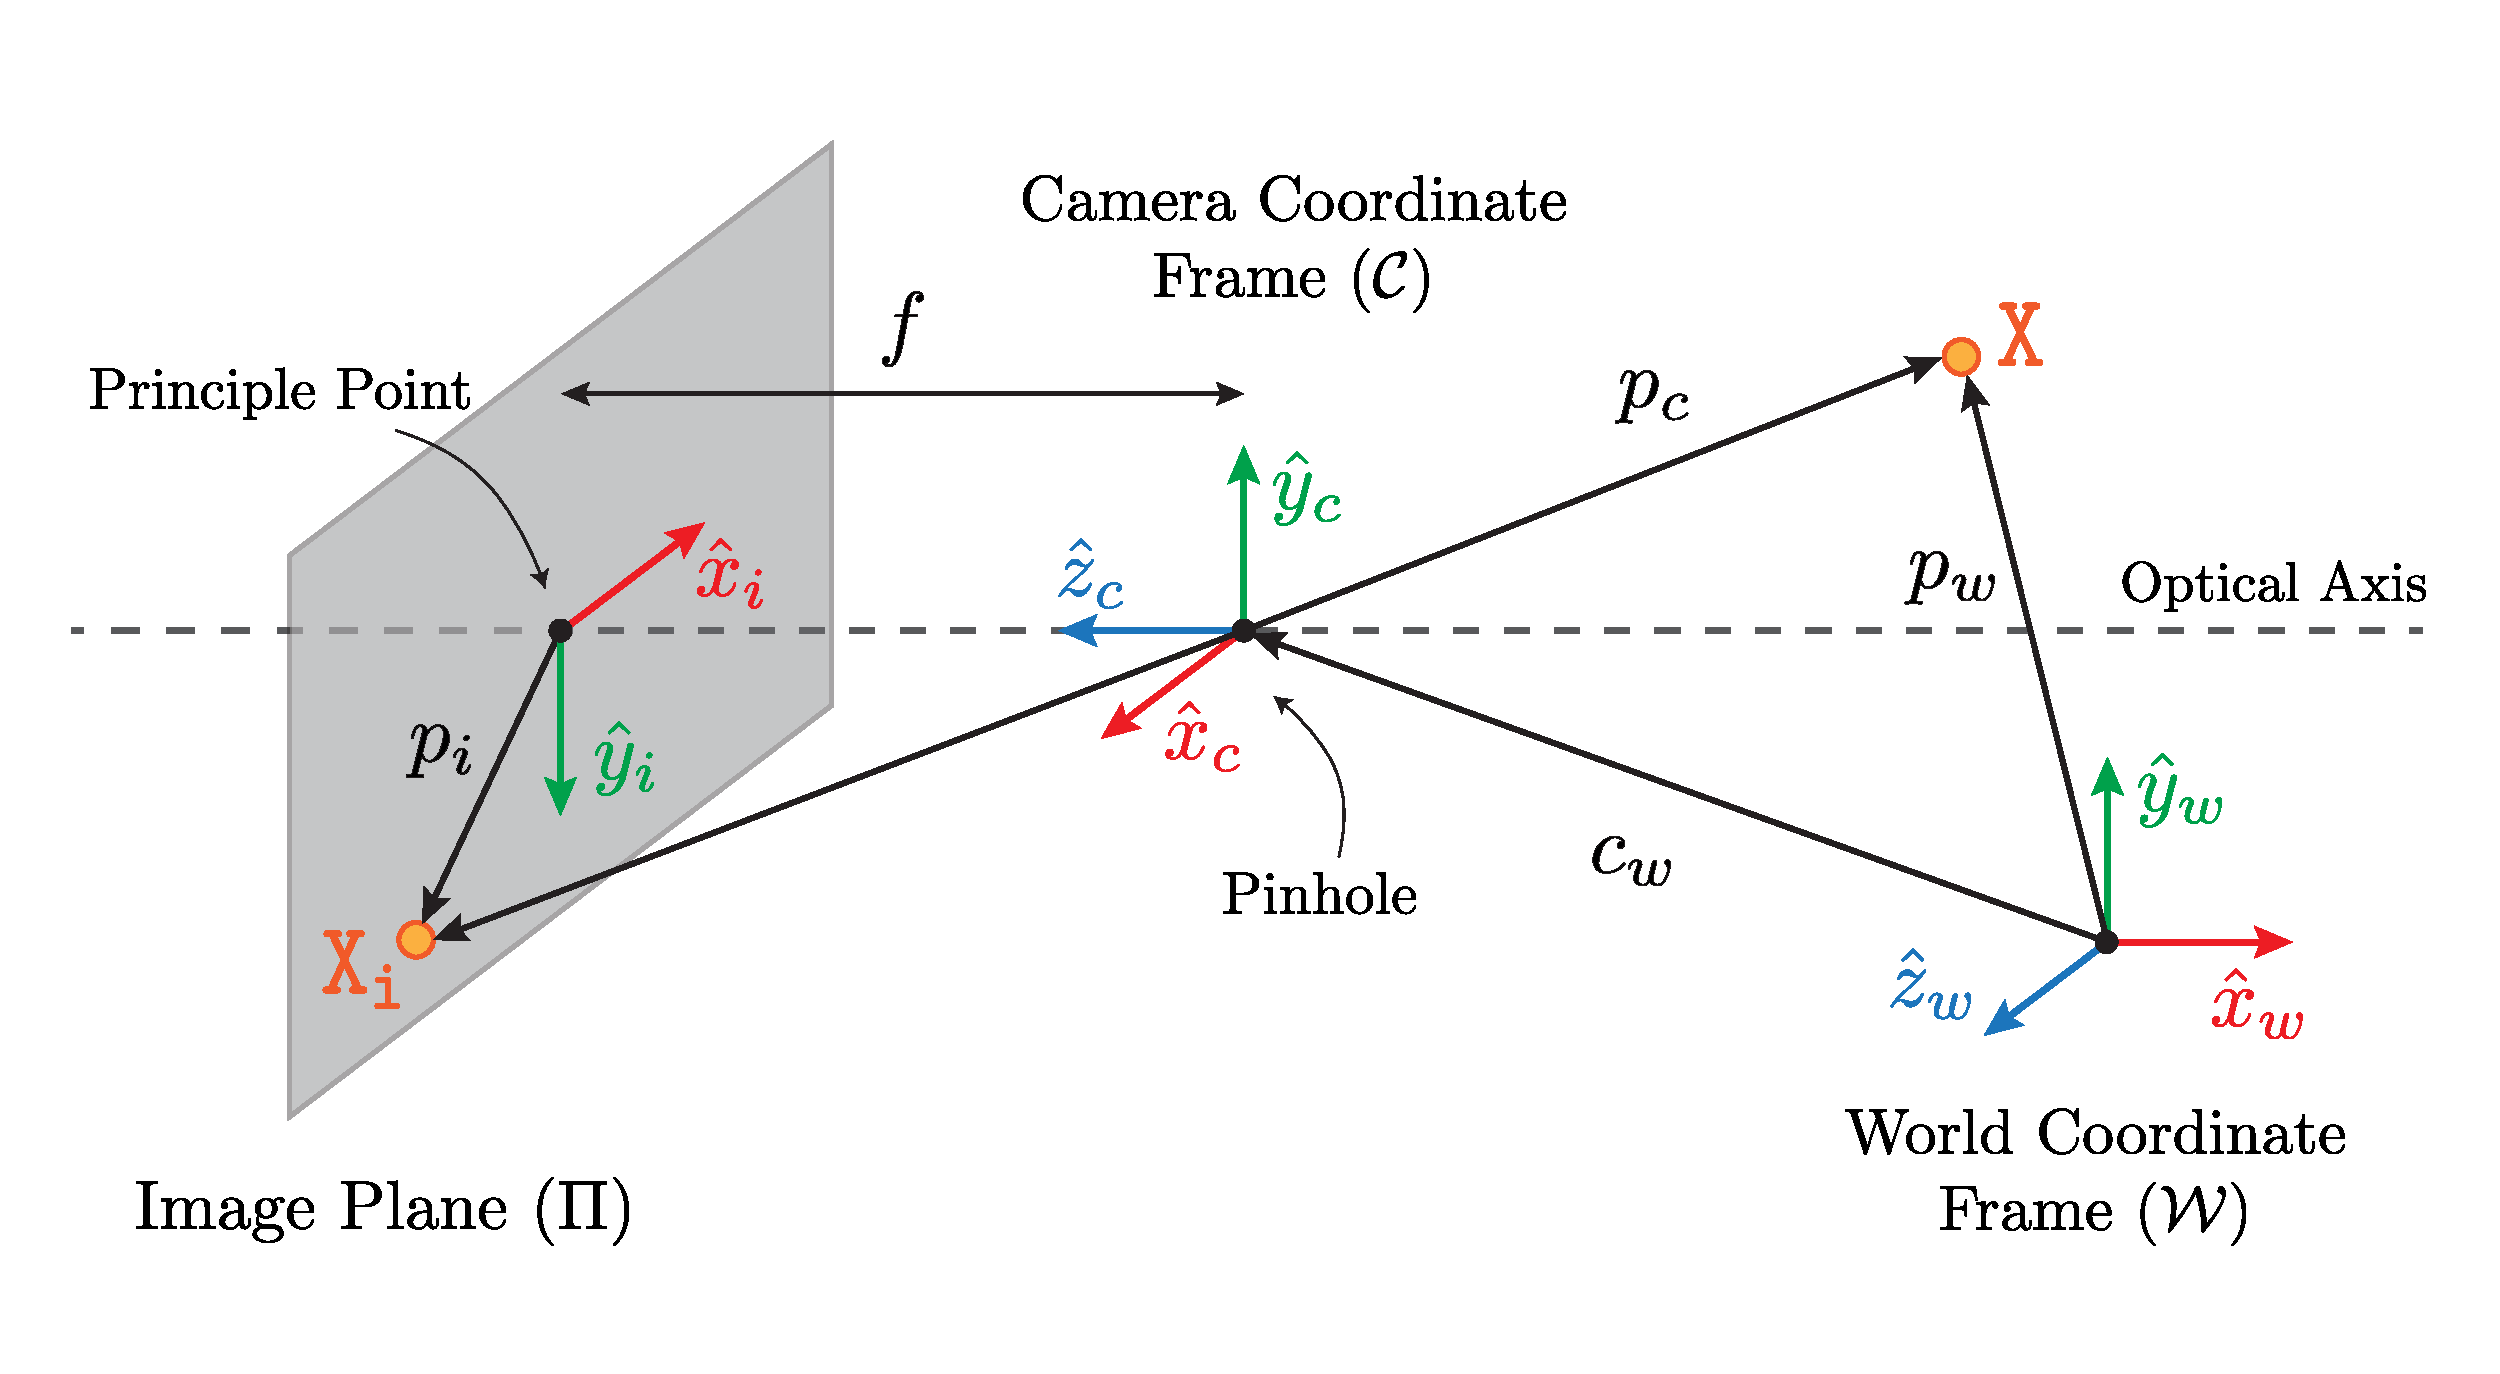
\includegraphics[width=\textwidth]{diagrams/imaging_model}
    \caption{Pinhole camera model.}
\end{figure}

For our camera model, we will introduce 4 different frames of reference, all of which :
\begin{itemize}[leftmargin=!, itemindent=-4ex]
    \item\textbf{World Coordinate Frame ($\boldsymbol{\mathcal{W}}$)}. Represents the 3D space of the scene being photographed, with respect to an origin which may be arbitrary and depends on the conventions chosen. Objects that are in the scene are defined with respect to this coordinate frame.
    \item\textbf{Camera Coordinate Frame ($\boldsymbol{\mathcal{C}}$)}. Represents the 3D space of the scene being photographed, but with respect to the pinhole (aperture) of the camera.
    \item\textbf{Image Coordinate Frame ($\boldsymbol{\Pi}$)}. 2D plane representing the image sensor plane of the camera. The origin is the principle point of the image sensor, where the optical axis intersects the image plane.
    \item\textbf{Pixel Coordinate Frame}. 2D plane representing the position of pixels on the image sensor. The Discrete version of the image coordinate frame, where c
\end{itemize}

The optical axis of a camera is an imaginary line which passes through the center of the aperture of the camera.





\begin{figure}[H]
    \centering
    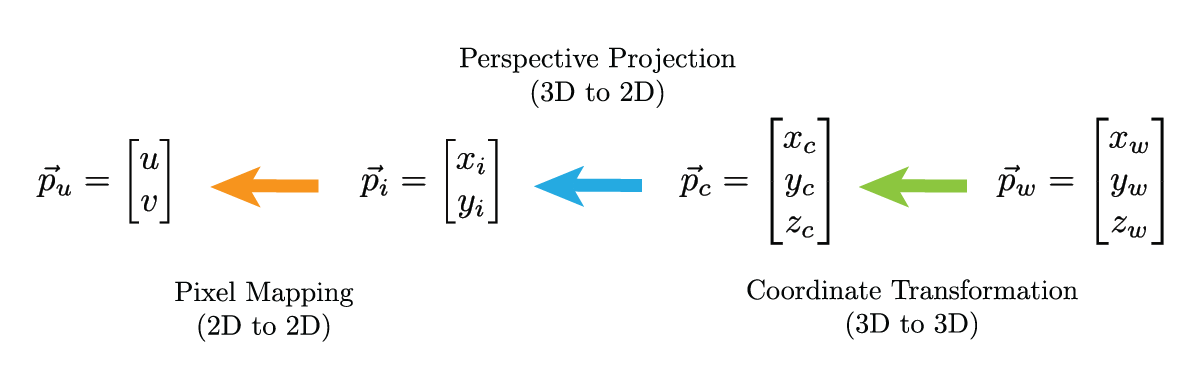
\includegraphics[width=0.9\textwidth]{diagrams/coord_conversions}
    \caption{Coordinate transformations.}
\end{figure}


\subsection{Intrinsic Parameters} \label{sec:intrinsics}

Intrinsic parameters describe the internal characteristics of the camera. In other words, it dictates how in the 3D space are projected onto the image plane, i.e. the relationship between the position of the point $\mathtt{X}$ to its projection on the image plane.

\begin{figure}[H]
    \centering
    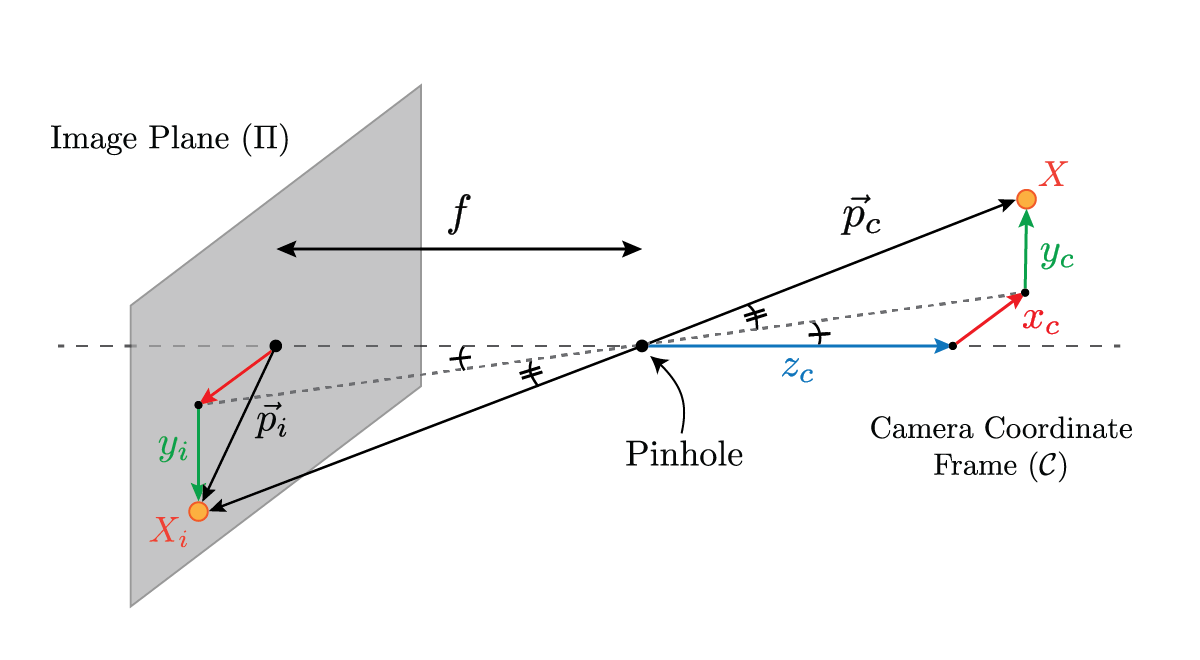
\includegraphics[width=0.9\textwidth]{diagrams/perspective_projection}
    \caption{Perspective projection of the point $\mathtt{X}$ onto the image plane $\Pi$.}
\end{figure}
When a straight line is drawn from $\mathtt{X}$ to its projection $\mathtt{X_i}$ through the aperture, it intersects the optical axis. Deconstructing this intersection in the $x$ and $y$ direction, pairs of similar triangles are formed, which relates $x_i$ to $x_c$ and $y_i$ to $y_c$.
\begin{figure}[H]
    \centering
    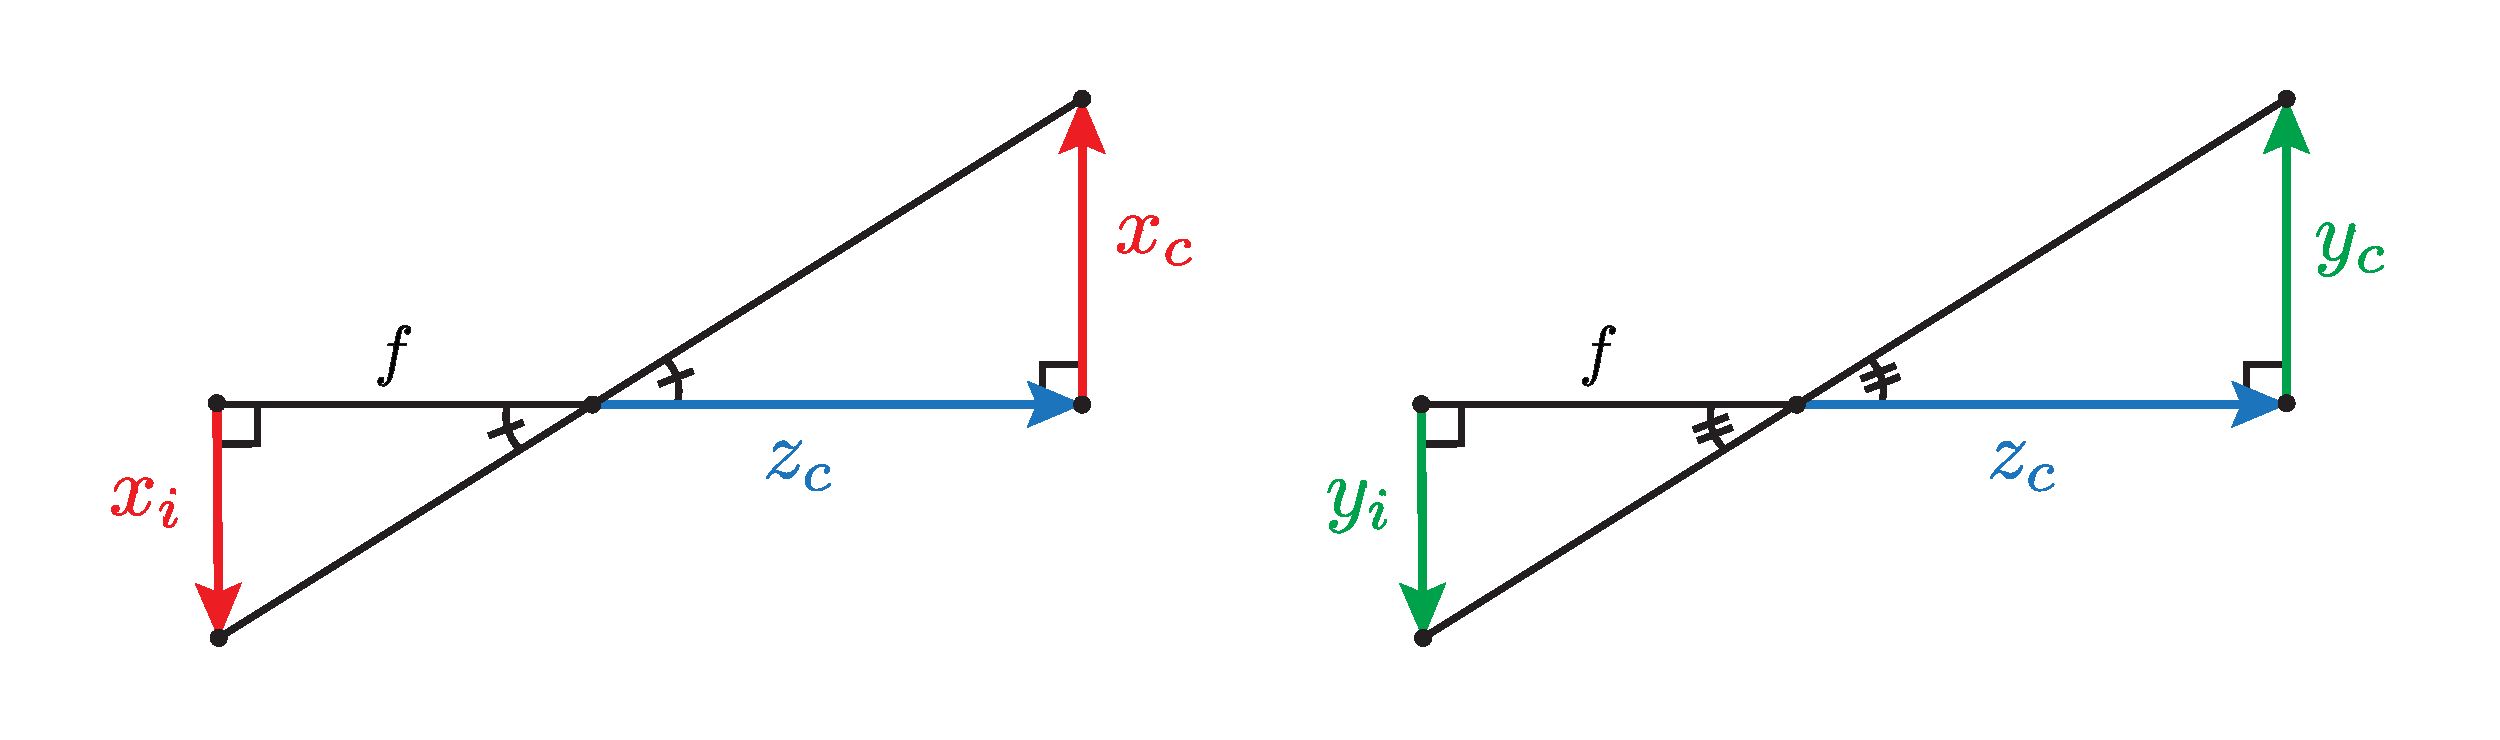
\includegraphics[width=\textwidth]{diagrams/similar_triangles}
    \caption{Similar triangles formed by perspective projection, which relate $x_i$ to $x_c$ and $y_i$ to $y_c$.} \label{fig:similar_triangles}
\end{figure}
\begin{subequations}
    \begin{gather}
        \frac{x_i}{f} = \frac{x_c}{z_c} \quad \Longrightarrow \quad x_i = f \frac{x_c}{z_c} \label{subeq:xi_result}\\
        \frac{y_i}{f} = \frac{y_c}{z_c} \quad \Longrightarrow \quad y_i = f \frac{y_c}{z_c} \label{subeq:yi_result}
    \end{gather}
\end{subequations}
Once the coordinates of the point projection, $(x_i, y_i)$, is known, we then need to convert it to actual pixel position of the point on the image, $(u, v)$. Pixel coordinates are measured in pixels, from the left-hand corner of the image. This is the convention that is typically followed in computer graphics. As such, there will be an offset in pixels, $(c_x, c_y)$, which represents the optical center of the image (i.e. the point at which the optical axis intersects the image plane). Additionally, the relationship between $(x_i, y_i)$ and $(u, v)$ is proportional, but they scale at different rates, as $(x_i, y_i)$ can be measured using any unit measurement, and can have negative and decimal values. On the other hand, $(u,v)$ are measured in discrete pixel value, which can different sizes depending on the camera used. As such, we define scaling factors, $m_x$ and $m_y$, be scaling factors which represent the pixel density of the image sensor in the $x$ and $y$ axes of the image sensor plane respectively.
\begin{figure}[H]
    \centering
    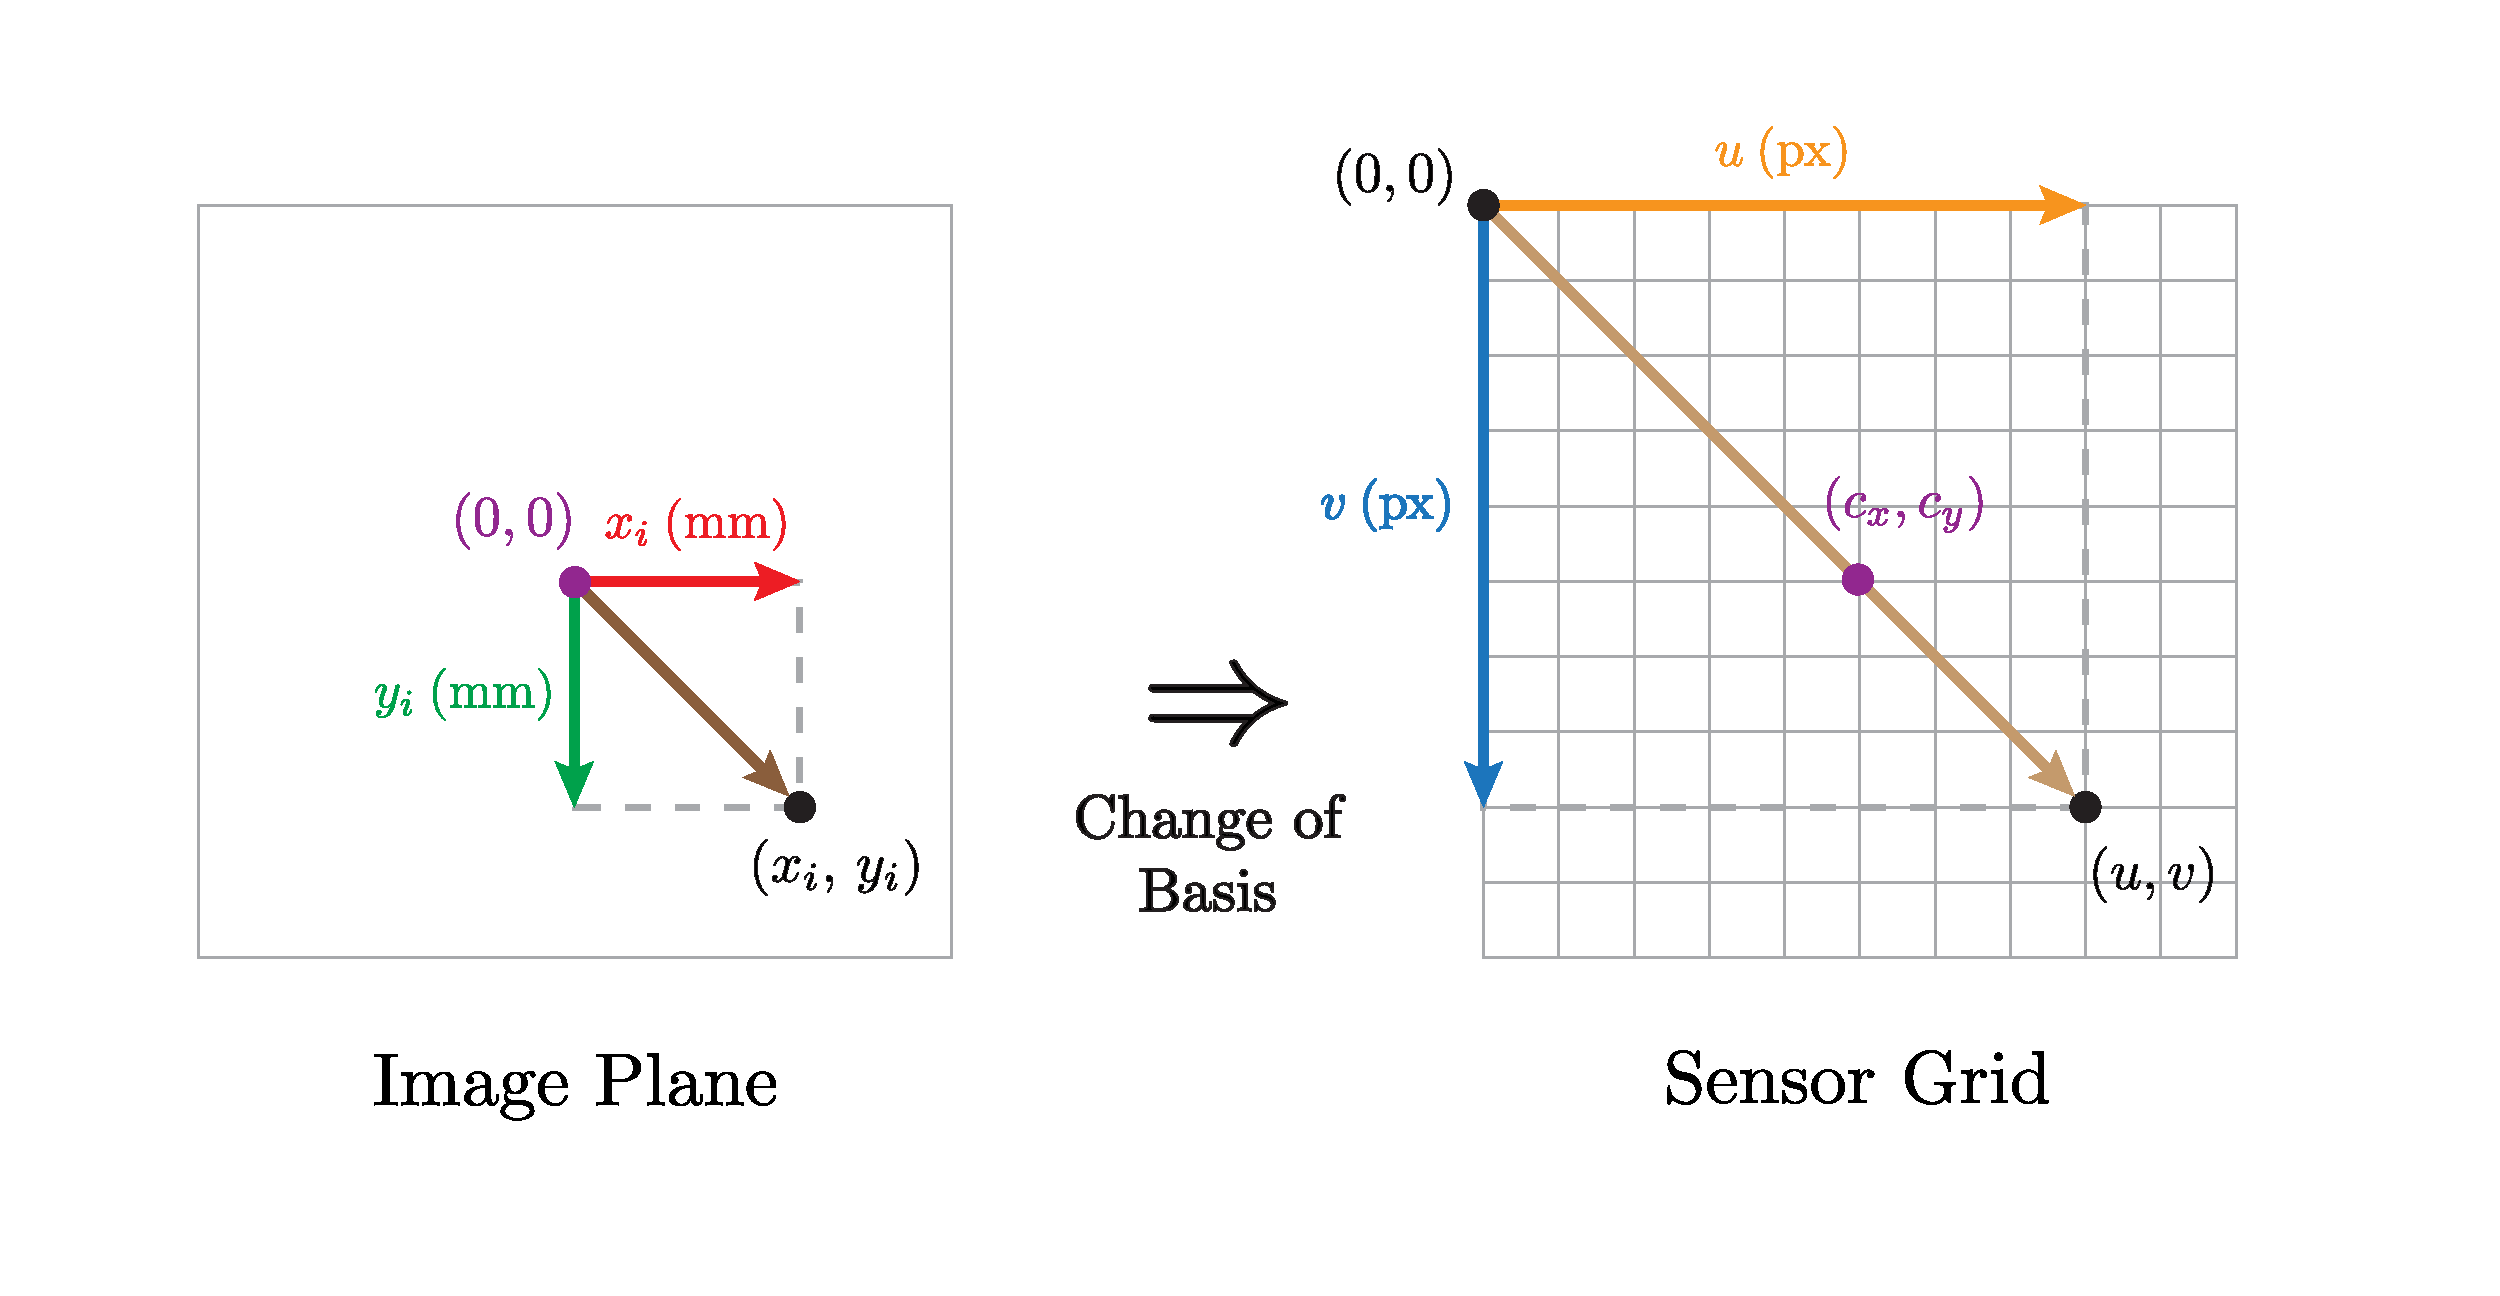
\includegraphics[width=\textwidth]{diagrams/sensor_grid}
    \caption{Conversion from image plane coordinates to sensor grid coordinates}
\end{figure}
Putting all the ideas above together, we can construct a set of linear parametric equations relating the pixel coordinates to their image coordinates thus:
\begin{align*}
    u = m_x x_i + c_x \\
    v = m_y y_i + c_y
\end{align*}
where $u,v \in \Integer^+_{\,*}$. Replacing $x_i$ and $y_i$ for the result we obtained from equations \ref{subeq:xi_result} and \ref{subeq:yi_result}, we get:
\begin{align*}
    u = m_x f \frac{x_c}{z_c} + c_x \\
    v = m_y f \frac{y_c}{z_c} + c_y
\end{align*}
This gives us a direct relationship between camera coordinates and their corresponding pixel coordinates. Since $m_x$, $m_y$, and $f$ are all unknowns, we can combine the products $m_x f$ and $m_y f$ into to $f_x$ and $f_y$ respectively. Under this new scheme, we define $f_x$ and $f_y$ as the horizontal and vertical focal lengths of camera.
\begin{gather}
    u = f_x \frac{x_c}{z_c} + c_x \\
    v = f_y \frac{y_c}{z_c} + c_y
\end{gather}
Multiply both sides of the equations by $z_c$.
\begin{subequations}
    \begin{gather*}
        z_c u = f_x x_c + z_c c_x \\
        z_c v = f_y y_c + z_c c_y
    \end{gather*}
\end{subequations}
Doing so allows us to express the relationship as a matrix transformation using homogenous coordinates, by letting $\widetilde{w} = z_c$.
\begin{equation}
    \begin{bmatrix}
        z_c u \\ z_c v \\ z_c
    \end{bmatrix}
    =
    \begin{bmatrix}
        f_x x_c + z_c c_x \\ f_y y_c + z_c c_y \\ z_c
    \end{bmatrix}
    =
    \underbrace{
        \begin{bmatrix}
            f_x & 0   & c_x \\
            0   & f_y & c_y \\
            0   & 0   & 1
        \end{bmatrix}
    }_{\mathlarger{K}}
    \begin{bmatrix}
        x_c \\ y_c \\ z_c
    \end{bmatrix}
\end{equation}
This can be represented simply with:
\begin{gather}
    k\,\widetilde{p}_i = K\, p_c \label{eq:pi}
\end{gather}
In this case, $K$ is what is known as the \emph{calibration matrix}. It is a matrix transformation which maps a point represented in the camera coordinate frame to the coordinates of their projection onto the sensor plane.

\subsection{Extrinsic Parameters} \label{sec:extrinsics}

Extrinsic parameters describe the orientation of the camera. As such, they can be used to describe the relationship between the position of a point in the world coordinate frame and its coordinates relative to the camera.

\begin{figure}[H]
    \centering
    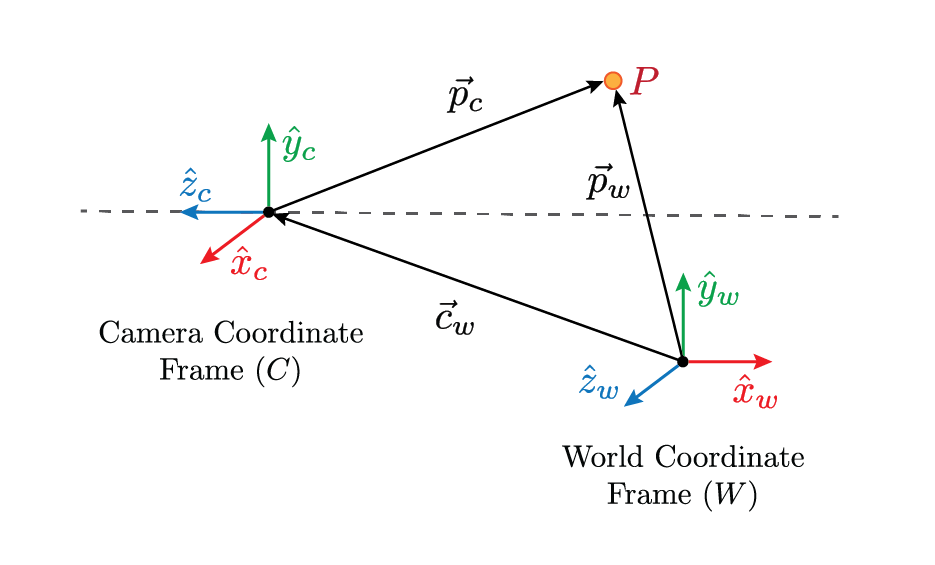
\includegraphics[width=0.9\textwidth]{diagrams/coord_transform}
    \caption{Coordinate transformation of $\mathtt{X}$ from the world coordinate frame to the camera coordinate frame.}
\end{figure}


There are two possible types of movement affecting the orientation of the camera: rotation and translation. The rotation of the camera can be described using a $3 \times 3$ rotational matrix:

\begin{equation}
    R =
    \begin{bmatrix}
        r_{11} & r_{12} & r_{13} \\
        r_{21} & r_{22} & r_{23} \\
        r_{31} & r_{32} & r_{33}
    \end{bmatrix}
\end{equation}

\noindent where:
\begin{itemize}
    \item Row 1: Unit vector representing $\hat{x}_c$ after rotation.
    \item Row 2: Unit vector representing $\hat{y}_c$ after rotation.
    \item Row 3: Unit vector representing $\hat{z}_c$ after rotation.
\end{itemize}
\begin{align}
    p_c & = R\,(p_w-c_w) \nonumber        \\
        & = R\,p_w -R\,c_w \label{eq:ext}
\end{align}
Replacing $R\,c_w$ with a vector $t$, where $t$ represents the translation of the camera from the origin, we can rewrite equation \ref{eq:ext}:
\begin{equation}
    p_c = R\,p_w + t
\end{equation}
This can be equivalently written as thus:
\begin{equation*}
    \begin{bmatrix}
        x_c \\ y_c \\ z_c
    \end{bmatrix}
    =
    \begin{bmatrix}
        r_{11} & r_{12} & r_{13} \\
        r_{21} & r_{22} & r_{23} \\
        r_{31} & r_{32} & r_{33}
    \end{bmatrix}
    \begin{bmatrix}
        x_w \\ y_w \\ z_w
    \end{bmatrix}
    +
    \begin{bmatrix}
        t_x \\ t_y \\ t_z
    \end{bmatrix}
\end{equation*}
When written like this, it is much easier to see that we can combine the parameters of $R$ and $t$ into one single $3 \times 4$ matrix, by expressing $p_w$ in homogenous coordinates.
\begin{equation}
    \begin{bmatrix}
        x_c \\ y_c \\ z_c
    \end{bmatrix}
    =
    \begin{bmatrix}
        r_{11} & r_{12} & r_{13} & t_x \\
        r_{21} & r_{22} & r_{23} & t_y \\
        r_{31} & r_{32} & r_{33} & t_z \\
    \end{bmatrix}
    \begin{bmatrix}
        x_w \\ y_w \\ z_w \\ 1
    \end{bmatrix}
\end{equation}
Thus, we arrive at the final equation:
\begin{equation}
    p_c=T\,\widetilde{p}_w\,, \qquad \text{with } T=[\,K\;|\;t\,] \label{eq:pc}
\end{equation}

